\section{Obtendo Ajuda}

Aprenda a usar bem os arquivos da Ajuda (“Help”). Muitas vezes, ao final de cada página da Ajuda, há exemplos úteis.  Role a página para baixo para conferi-los, mesmo que (ou especialmente se) você não entendeu completamente as explicações do texto. Você pode rodar os exemplos diretamente do browser da Ajuda ou você pode copiar e colar o código em uma nova janela para brincar com ele. 

Selecione qualquer classe ou método válidos no seu código de SuperCollider (um duplo-clique na palavra irá selecioná-la) e aperte [ctrl+D] para abrir o arquivo de Help correspondente. Se você selecionar o nome de uma classe (por exemplo, \texttt{MouseX}), você será direcionado para o arquivo de Ajuda da classe. Se você selecionar um método (por exemplo, peça ajuda do método \texttt{scramble}. \footnote{Atenção: O SuperCollider vai mostrar em azul qualquer palavra que começa com uma letra maiúscula. Isso significa que a cor azul \emph{não garante} que a palavra esteja livre de erros: por exemplo, se você digitar Sinosc (com o “o” minúsculo incorreto), ainda assim a palavra aparece em azul.}

Outras maneiras de explorar os arquivos de Ajuda da IDE do SuperCollider são os links “Browse” (“Navegar”) e “Search” (“Pesquisar”). Use o Browse para navegar os arquivos por categorias e o Search para pesquisar palavras em todos os arquivos de Ajuda.
Nota importante sobre o Browser de Ajuda na IDE do SuperCollider:

\begin{itemize}
\item Use o campo superior direito (onde se lê “Find…”) para procurar palavras específicas \emph{dentro do arquivo de Help que está aberto} (como você usaria um “find” para localizar algo em um website);
\item Use o link “Search” (à direita de “Browse”) para procurar texto \emph{em todos os arquivos de Ajuda}.
\end{itemize}

Quando você abrir o primeiro parênteses para adicionar argumentos para um método específico, o SC mostra uma pequena “dica de ajuda” para mostrar quais são os argumentos esperados. Por exemplo, digite o início de uma linha que você vê na figura \ref{fig:tooltip}. Logo depois de abrir o primeiro parênteses, a dica mostra que os argumentos para um \texttt{SinOsc.ar} são \texttt{freq}, \texttt{phase}, \texttt{mul} e \texttt{add}. Também aparecem os valores padrão. Esta é exatamente a mesma informação que você obteria no arquivo de Ajuda do \texttt{SinOsc}. Se a dica de ajuda desapareceu, você pode trazê-la de volta com [ctrl+Shift+Espaço].

\begin{figure}[h]
\centerline{\framebox{
	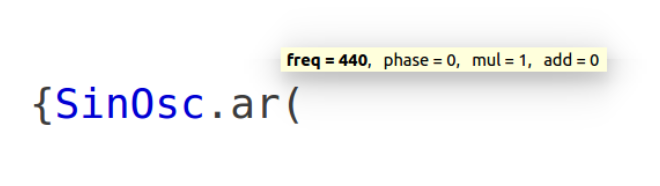
\includegraphics[scale=0.3]{fig-help-tooltip-crop.png}}}
\caption{Informação útil é mostrada conforme você vai digitando.}
\label{fig:tooltip}
\end{figure}

Outro atalho: se você quiser explicitamente nomear seus argumentos (como \texttt{SinOsc.ar(freq: 890)}), experimente apertar a tecla Tab logo depois de abrir os parênteses. O SC vai autocompletar para você com o nome do argumento correto, na ordem, à medida que você digita (aperte Tab depois da vírgula para os nomes dos argumentos subsequentes).

\bigskip
\todo[inline, color=green!40]{ 
DICA: Crie uma pasta com seus próprios “arquivos pessoais de ajuda”. Sempre que você descobrir um novo truque ou aprender um novo objeto, escreva um exemplo simples com explicações em suas próprias palavras e salve-o para o futuro. Isso pode ser útil daqui um mês ou um ano.

}
\bigskip

Os mesmos arquivos de Ajuda podem ser também encontrados onlin \url{http://doc.sccode.org/}.
